\documentclass[twoside]{book}

% Packages required by doxygen
\usepackage{fixltx2e}
\usepackage{calc}
\usepackage{doxygen}
\usepackage[export]{adjustbox} % also loads graphicx
\usepackage{graphicx}
\usepackage[utf8]{inputenc}
\usepackage{makeidx}
\usepackage{multicol}
\usepackage{multirow}
\PassOptionsToPackage{warn}{textcomp}
\usepackage{textcomp}
\usepackage[nointegrals]{wasysym}
\usepackage[table]{xcolor}

% Font selection
\usepackage[T1]{fontenc}
\usepackage[scaled=.90]{helvet}
\usepackage{courier}
\usepackage{amssymb}
\usepackage{sectsty}
\renewcommand{\familydefault}{\sfdefault}
\allsectionsfont{%
  \fontseries{bc}\selectfont%
  \color{darkgray}%
}
\renewcommand{\DoxyLabelFont}{%
  \fontseries{bc}\selectfont%
  \color{darkgray}%
}
\newcommand{\+}{\discretionary{\mbox{\scriptsize$\hookleftarrow$}}{}{}}

% Page & text layout
\usepackage{geometry}
\geometry{%
  a4paper,%
  top=2.5cm,%
  bottom=2.5cm,%
  left=2.5cm,%
  right=2.5cm%
}
\tolerance=750
\hfuzz=15pt
\hbadness=750
\setlength{\emergencystretch}{15pt}
\setlength{\parindent}{0cm}
\setlength{\parskip}{3ex plus 2ex minus 2ex}
\makeatletter
\renewcommand{\paragraph}{%
  \@startsection{paragraph}{4}{0ex}{-1.0ex}{1.0ex}{%
    \normalfont\normalsize\bfseries\SS@parafont%
  }%
}
\renewcommand{\subparagraph}{%
  \@startsection{subparagraph}{5}{0ex}{-1.0ex}{1.0ex}{%
    \normalfont\normalsize\bfseries\SS@subparafont%
  }%
}
\makeatother

% Headers & footers
\usepackage{fancyhdr}
\pagestyle{fancyplain}
\fancyhead[LE]{\fancyplain{}{\bfseries\thepage}}
\fancyhead[CE]{\fancyplain{}{}}
\fancyhead[RE]{\fancyplain{}{\bfseries\leftmark}}
\fancyhead[LO]{\fancyplain{}{\bfseries\rightmark}}
\fancyhead[CO]{\fancyplain{}{}}
\fancyhead[RO]{\fancyplain{}{\bfseries\thepage}}
\fancyfoot[LE]{\fancyplain{}{}}
\fancyfoot[CE]{\fancyplain{}{}}
\fancyfoot[RE]{\fancyplain{}{\bfseries\scriptsize Generated by Doxygen }}
\fancyfoot[LO]{\fancyplain{}{\bfseries\scriptsize Generated by Doxygen }}
\fancyfoot[CO]{\fancyplain{}{}}
\fancyfoot[RO]{\fancyplain{}{}}
\renewcommand{\footrulewidth}{0.4pt}
\renewcommand{\chaptermark}[1]{%
  \markboth{#1}{}%
}
\renewcommand{\sectionmark}[1]{%
  \markright{\thesection\ #1}%
}

% Indices & bibliography
\usepackage{natbib}
\usepackage[titles]{tocloft}
\setcounter{tocdepth}{3}
\setcounter{secnumdepth}{5}
\makeindex

% Hyperlinks (required, but should be loaded last)
\usepackage{ifpdf}
\ifpdf
  \usepackage[pdftex,pagebackref=true]{hyperref}
\else
  \usepackage[ps2pdf,pagebackref=true]{hyperref}
\fi
\hypersetup{%
  colorlinks=true,%
  linkcolor=blue,%
  citecolor=blue,%
  unicode%
}

% Custom commands
\newcommand{\clearemptydoublepage}{%
  \newpage{\pagestyle{empty}\cleardoublepage}%
}

\usepackage{caption}
\captionsetup{labelsep=space,justification=centering,font={bf},singlelinecheck=off,skip=4pt,position=top}

%===== C O N T E N T S =====

\begin{document}

% Titlepage & ToC
\hypersetup{pageanchor=false,
             bookmarksnumbered=true,
             pdfencoding=unicode
            }
\pagenumbering{alph}
\begin{titlepage}
\vspace*{7cm}
\begin{center}%
{\Large M\+CS \\[1ex]\large 3 }\\
\vspace*{1cm}
{\large Generated by Doxygen 1.8.13}\\
\end{center}
\end{titlepage}
\clearemptydoublepage
\pagenumbering{roman}
\tableofcontents
\clearemptydoublepage
\pagenumbering{arabic}
\hypersetup{pageanchor=true}

%--- Begin generated contents ---
\chapter{R\+E\+A\+D\+ME}
\label{md__r_e_a_d_m_e}
\Hypertarget{md__r_e_a_d_m_e}
projet M\+CS Valentine Petit Valentin Blet

protocol\+:

Un serveur général est lancé (adress ip fixe) Les clients se connectent au serveur Le serveur redirige les messages envoyés par chaque client aux autres clients 
\chapter{Class Index}
\section{Class List}
Here are the classes, structs, unions and interfaces with brief descriptions\+:\begin{DoxyCompactList}
\item\contentsline{section}{\hyperlink{struct_t___client}{T\+\_\+\+Client} }{\pageref{struct_t___client}}{}
\end{DoxyCompactList}

\chapter{File Index}
\section{File List}
Here is a list of all documented files with brief descriptions\+:\begin{DoxyCompactList}
\item\contentsline{section}{\hyperlink{_tchatstream_8c}{Tchatstream.\+c} \\*Programme utilisant les sockets pour réaliser un serveur multi client }{\pageref{_tchatstream_8c}}{}
\end{DoxyCompactList}

\chapter{Class Documentation}
\hypertarget{struct_t___client}{}\section{T\+\_\+\+Client Struct Reference}
\label{struct_t___client}\index{T\+\_\+\+Client@{T\+\_\+\+Client}}
\subsection*{Public Attributes}
\begin{DoxyCompactItemize}
\item 
\mbox{\Hypertarget{struct_t___client_a37311cdecddea203b6856f2e9120cf32}\label{struct_t___client_a37311cdecddea203b6856f2e9120cf32}} 
int {\bfseries Nb\+Client}
\item 
\mbox{\Hypertarget{struct_t___client_aa3f3ad3f2eaa285e098e19a3800c9ecc}\label{struct_t___client_aa3f3ad3f2eaa285e098e19a3800c9ecc}} 
char $\ast$ {\bfseries pseudo}
\item 
\mbox{\Hypertarget{struct_t___client_ae23acc3d90699e37a485e898a4465c6b}\label{struct_t___client_ae23acc3d90699e37a485e898a4465c6b}} 
char $\ast$ {\bfseries I\+Pclient}
\item 
\mbox{\Hypertarget{struct_t___client_a6d96a375cc128bad3093f9274b1a9314}\label{struct_t___client_a6d96a375cc128bad3093f9274b1a9314}} 
char $\ast$ {\bfseries port\+Client}
\end{DoxyCompactItemize}


The documentation for this struct was generated from the following files\+:\begin{DoxyCompactItemize}
\item 
essai.\+c\item 
\hyperlink{_tchatstream_8c}{Tchatstream.\+c}\end{DoxyCompactItemize}

\chapter{File Documentation}
\hypertarget{_tchatstream_8c}{}\section{Tchatstream.\+c File Reference}
\label{_tchatstream_8c}\index{Tchatstream.\+c@{Tchatstream.\+c}}


Programme utilisant les sockets pour réaliser un serveur multi client.  


{\ttfamily \#include $<$stdio.\+h$>$}\newline
{\ttfamily \#include $<$string.\+h$>$}\newline
{\ttfamily \#include $<$stdlib.\+h$>$}\newline
{\ttfamily \#include $<$unistd.\+h$>$}\newline
{\ttfamily \#include $<$netdb.\+h$>$}\newline
{\ttfamily \#include $<$sys/socket.\+h$>$}\newline
{\ttfamily \#include $<$sys/time.\+h$>$}\newline
{\ttfamily \#include $<$netinet/in.\+h$>$}\newline
{\ttfamily \#include $<$arpa/inet.\+h$>$}\newline
{\ttfamily \#include $<$pthread.\+h$>$}\newline
Include dependency graph for Tchatstream.\+c\+:
\nopagebreak
\begin{figure}[H]
\begin{center}
\leavevmode
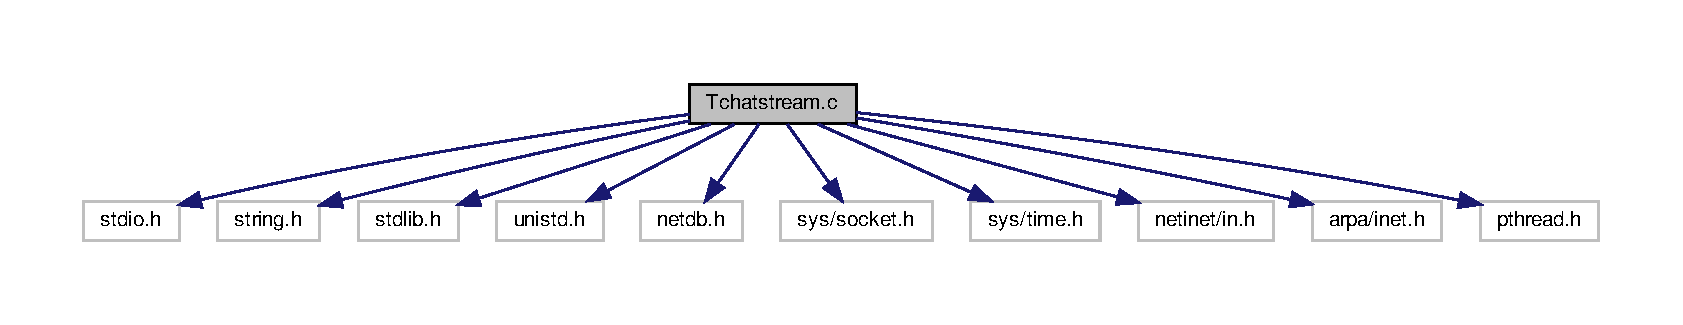
\includegraphics[width=350pt]{_tchatstream_8c__incl}
\end{center}
\end{figure}
\subsection*{Classes}
\begin{DoxyCompactItemize}
\item 
struct \hyperlink{struct_t___client}{T\+\_\+\+Client}
\end{DoxyCompactItemize}
\subsection*{Macros}
\begin{DoxyCompactItemize}
\item 
\mbox{\Hypertarget{_tchatstream_8c_ad3fe337408f16c132c895f2b59326410}\label{_tchatstream_8c_ad3fe337408f16c132c895f2b59326410}} 
\#define {\bfseries C\+H\+E\+CK}(sts,  msg)~if ((sts)==-\/1) \{perror(msg); exit(-\/1);\}
\item 
\mbox{\Hypertarget{_tchatstream_8c_a818b4345f7c175a751c056a83ccdfe2d}\label{_tchatstream_8c_a818b4345f7c175a751c056a83ccdfe2d}} 
\#define {\bfseries N\+B\+C\+L\+I\+E\+NT}~5
\item 
\mbox{\Hypertarget{_tchatstream_8c_a4b70916bdf28ed7afd94e4fb98230a90}\label{_tchatstream_8c_a4b70916bdf28ed7afd94e4fb98230a90}} 
\#define {\bfseries M\+A\+X\+\_\+\+B\+U\+FF}~512
\item 
\mbox{\Hypertarget{_tchatstream_8c_a63cc51955a32e949e602d322d28762ec}\label{_tchatstream_8c_a63cc51955a32e949e602d322d28762ec}} 
\#define {\bfseries P\+O\+R\+T\+\_\+\+S\+RV}~15130
\item 
\mbox{\Hypertarget{_tchatstream_8c_a9283392aacb3aac1b7a17d1c7d047c16}\label{_tchatstream_8c_a9283392aacb3aac1b7a17d1c7d047c16}} 
\#define {\bfseries A\+D\+D\+R\+\_\+\+S\+RV}~\char`\"{}127.\+0.\+0.\+24\char`\"{}
\item 
\mbox{\Hypertarget{_tchatstream_8c_a82acb32225c05e9aa4c524c40bc5852a}\label{_tchatstream_8c_a82acb32225c05e9aa4c524c40bc5852a}} 
\#define {\bfseries M\+A\+X\+\_\+\+C\+H\+AR}~512
\item 
\mbox{\Hypertarget{_tchatstream_8c_a3f40d4c5c9e3ece45fdda52d72046378}\label{_tchatstream_8c_a3f40d4c5c9e3ece45fdda52d72046378}} 
\#define {\bfseries N\+O\+M\+\_\+\+F\+I\+C\+H\+I\+ER}~\char`\"{}enregistrement.\+txt\char`\"{}
\end{DoxyCompactItemize}
\subsection*{Typedefs}
\begin{DoxyCompactItemize}
\item 
\mbox{\Hypertarget{_tchatstream_8c_a8e74e7fdb6a26dff7d96f9e41ec4821a}\label{_tchatstream_8c_a8e74e7fdb6a26dff7d96f9e41ec4821a}} 
typedef char {\bfseries message\+\_\+t}\mbox{[}M\+A\+X\+\_\+\+B\+U\+FF\mbox{]}
\end{DoxyCompactItemize}
\subsection*{Functions}
\begin{DoxyCompactItemize}
\item 
void \hyperlink{_tchatstream_8c_aef12aca1965ea852ad5c36baf00d4901}{fermeture} (void)
\begin{DoxyCompactList}\small\item\em Cette fonction permet de fermer la socket d\textquotesingle{}écoute global. \end{DoxyCompactList}\item 
\mbox{\Hypertarget{_tchatstream_8c_abec39e04f4b20e160e4c29e6887814ff}\label{_tchatstream_8c_abec39e04f4b20e160e4c29e6887814ff}} 
void {\bfseries init} (\hyperlink{struct_t___client}{T\+\_\+\+Client} $\ast$clt, int Nb\+Client)
\item 
\mbox{\Hypertarget{_tchatstream_8c_a767631cccf66570b301ecfab29b17307}\label{_tchatstream_8c_a767631cccf66570b301ecfab29b17307}} 
void {\bfseries Affiche} (\hyperlink{struct_t___client}{T\+\_\+\+Client} $\ast$clt)
\item 
int \hyperlink{_tchatstream_8c_afa2aacb693bac10c6c1ebdfe9ac736dd}{comparer} (const char truck1\mbox{[}$\,$\mbox{]}, const char truck2\mbox{[}$\,$\mbox{]})
\begin{DoxyCompactList}\small\item\em Cette fonction permet de comparer les chaines passer en parametre. \end{DoxyCompactList}\item 
int \hyperlink{_tchatstream_8c_a4498b4dd750edba3dee33be6c5c1c0a2}{taille\+Chaine} (const char truck\mbox{[}$\,$\mbox{]})
\begin{DoxyCompactList}\small\item\em Cette fonction permet de calculer la taille de la chaine passer en parametre. \end{DoxyCompactList}\item 
void \hyperlink{_tchatstream_8c_a4d705207ad5dc030f95aa9de8d262d7f}{ecrire\+Fichier\+Enregistrement} (char $\ast$pseudo, char $\ast$Ip\+Client, int Port\+Client)
\begin{DoxyCompactList}\small\item\em Cette fonction est appele une fois le client connecter au serveur, elle permet de renseigner dans le fichier enregistrement.\+txt, le port du Client et l\textquotesingle{}Ip du client et son pseudo. \end{DoxyCompactList}\item 
\mbox{\Hypertarget{_tchatstream_8c_aa9ba8f3bc99c46cc8f864f0924cb031a}\label{_tchatstream_8c_aa9ba8f3bc99c46cc8f864f0924cb031a}} 
void {\bfseries lire\+Enregistrement} (\hyperlink{struct_t___client}{T\+\_\+\+Client} $\ast$clt, int nb\+Ligne)
\item 
void \hyperlink{_tchatstream_8c_a583fcca3e259924303d730b7c0d7fee5}{dial\+Clt2\+Srv} (int sad)
\begin{DoxyCompactList}\small\item\em Cette fonction permet le dialogue entre un client et le serveur. \end{DoxyCompactList}\item 
char \hyperlink{_tchatstream_8c_a83ec72c6be4de3e88c20abd80e8adafc}{dial\+Srv2\+Clt} (int sd, struct sockaddr\+\_\+in $\ast$clt\+Adr)
\begin{DoxyCompactList}\small\item\em Cette fonction permet le dialogue du serveur au client. \end{DoxyCompactList}\item 
void \hyperlink{_tchatstream_8c_a1684b65f61b6f9ebbdf0d89fc52b9cdf}{dial\+Clt2\+Clt} (char msg)
\begin{DoxyCompactList}\small\item\em Cette fonction recupere les infos des différents clients et leur transmet msg. \end{DoxyCompactList}\item 
int \hyperlink{_tchatstream_8c_afe7336714349079061a241cbe76b6421}{accept\+Clt} (int socket\+Ecoute, struct sockaddr\+\_\+in $\ast$clt\+Adr)
\begin{DoxyCompactList}\small\item\em Cette fonction permet d\textquotesingle{}accepter la connexion d\textquotesingle{}un client au serveur. \end{DoxyCompactList}\item 
\mbox{\Hypertarget{_tchatstream_8c_adb723d4c0b7a57a31a2de35be952a566}\label{_tchatstream_8c_adb723d4c0b7a57a31a2de35be952a566}} 
void {\bfseries serveur} ()
\item 
void \hyperlink{_tchatstream_8c_a7d0f00f54686b7ecfb1c73edca3ee4f4}{client} ()
\begin{DoxyCompactList}\small\item\em Fonction principale du mode client permet de mettre en place ( session\+Clt , connect\+Srv, dial\+Clt2\+Srv) \end{DoxyCompactList}\item 
\mbox{\Hypertarget{_tchatstream_8c_ae66f6b31b5ad750f1fe042a706a4e3d4}\label{_tchatstream_8c_ae66f6b31b5ad750f1fe042a706a4e3d4}} 
int {\bfseries main} ()
\item 
char $\ast$ \hyperlink{_tchatstream_8c_a79152f9ab9afe11e9cd97d58b2b6f89d}{decoupe\+Lire} (char $\ast$chaine)
\begin{DoxyCompactList}\small\item\em Cette fonction permet de comparer les chaines passer en parametre. \end{DoxyCompactList}\item 
int \hyperlink{_tchatstream_8c_ae6926c1c561f7ba5bcfa1ef13c267763}{session\+Srv} ()
\begin{DoxyCompactList}\small\item\em Cette fonction permet d\textquotesingle{}initialiser le serveur elle cree la socket d\textquotesingle{}ecoute puis l\textquotesingle{}associe a l\textquotesingle{}adresse ip et la met sur ecoute. \end{DoxyCompactList}\item 
void $\ast$ \hyperlink{_tchatstream_8c_aa039bbf344b8e5632f8cad0a70c22e00}{Thread\+Dialogue} (int socket\+Ecoute)
\begin{DoxyCompactList}\small\item\em Cette fonction permet le dialogue entre le client et le serveur et le envoie un message a tous les clients. \end{DoxyCompactList}\item 
int \hyperlink{_tchatstream_8c_add818693ace912c7fb49a09c31731c14}{session\+Clt} ()
\begin{DoxyCompactList}\small\item\em Cette fonction permet l\textquotesingle{}initialisation de la socket client. \end{DoxyCompactList}\item 
void \hyperlink{_tchatstream_8c_a2566f9a74b8d7ad785145f8002bf4a46}{connect\+Srv} (int sad)
\begin{DoxyCompactList}\small\item\em Cette fonction permet la connexion avec le serveur. \end{DoxyCompactList}\end{DoxyCompactItemize}
\subsection*{Variables}
\begin{DoxyCompactItemize}
\item 
\mbox{\Hypertarget{_tchatstream_8c_a206dbd65265d3da1bf018ba1b54b83b5}\label{_tchatstream_8c_a206dbd65265d3da1bf018ba1b54b83b5}} 
pthread\+\_\+t {\bfseries tid} \mbox{[}N\+B\+C\+L\+I\+E\+NT\mbox{]}
\item 
\mbox{\Hypertarget{_tchatstream_8c_ac4698a25ae5af5a55386151374fed504}\label{_tchatstream_8c_ac4698a25ae5af5a55386151374fed504}} 
int {\bfseries socket\+Ecoute}
\item 
\mbox{\Hypertarget{_tchatstream_8c_ae0d46a978d5cd6707411f276ad869b9c}\label{_tchatstream_8c_ae0d46a978d5cd6707411f276ad869b9c}} 
pid\+\_\+t {\bfseries pid}
\end{DoxyCompactItemize}


\subsection{Detailed Description}
Programme utilisant les sockets pour réaliser un serveur multi client. 

\begin{DoxyAuthor}{Author}
Valentine Petit et Valentin Blet Le3 T\+DA
\end{DoxyAuthor}
\begin{DoxyDate}{Date}
début \+: 08 janvier fin \+: 28 janvier
\end{DoxyDate}
\begin{DoxyVersion}{Version}
3.\+0
\begin{DoxyItemize}
\item 
\end{DoxyItemize}
\end{DoxyVersion}
\begin{DoxyRemark}{Remarks}
Le fichier doit être compiler avec -\/\+D\+S\+E\+R\+V\+E\+UR pour être executer en temps que serveur et -\/\+D\+C\+L\+I\+E\+NT pour être executer en temps que client. Il faut aussi ajouter -\/lpthread car nous utilisons les threads 
\end{DoxyRemark}


\subsection{Function Documentation}
\mbox{\Hypertarget{_tchatstream_8c_afe7336714349079061a241cbe76b6421}\label{_tchatstream_8c_afe7336714349079061a241cbe76b6421}} 
\index{Tchatstream.\+c@{Tchatstream.\+c}!accept\+Clt@{accept\+Clt}}
\index{accept\+Clt@{accept\+Clt}!Tchatstream.\+c@{Tchatstream.\+c}}
\subsubsection{\texorpdfstring{accept\+Clt()}{acceptClt()}}
{\footnotesize\ttfamily int accept\+Clt (\begin{DoxyParamCaption}\item[{int}]{socket\+Ecoute,  }\item[{struct sockaddr\+\_\+in $\ast$}]{clt\+Adr }\end{DoxyParamCaption})}



Cette fonction permet d\textquotesingle{}accepter la connexion d\textquotesingle{}un client au serveur. 


\begin{DoxyParams}{Parameters}
{\em int} & socket\+Ecoute la socket d\textquotesingle{}ecoute\\
\hline
{\em struct} & sockaddr\+\_\+in $\ast$clt\+Adr la socket du client\\
\hline
\end{DoxyParams}
\begin{DoxyReturn}{Returns}
socket\+Dialogue la socket de dialogue 
\end{DoxyReturn}
\mbox{\Hypertarget{_tchatstream_8c_a7d0f00f54686b7ecfb1c73edca3ee4f4}\label{_tchatstream_8c_a7d0f00f54686b7ecfb1c73edca3ee4f4}} 
\index{Tchatstream.\+c@{Tchatstream.\+c}!client@{client}}
\index{client@{client}!Tchatstream.\+c@{Tchatstream.\+c}}
\subsubsection{\texorpdfstring{client()}{client()}}
{\footnotesize\ttfamily void client (\begin{DoxyParamCaption}{ }\end{DoxyParamCaption})}



Fonction principale du mode client permet de mettre en place ( session\+Clt , connect\+Srv, dial\+Clt2\+Srv) 


\begin{DoxyParams}{Parameters}
{\em aucun} & \\
\hline
\end{DoxyParams}
\begin{DoxyReturn}{Returns}
rien 
\end{DoxyReturn}
\mbox{\Hypertarget{_tchatstream_8c_afa2aacb693bac10c6c1ebdfe9ac736dd}\label{_tchatstream_8c_afa2aacb693bac10c6c1ebdfe9ac736dd}} 
\index{Tchatstream.\+c@{Tchatstream.\+c}!comparer@{comparer}}
\index{comparer@{comparer}!Tchatstream.\+c@{Tchatstream.\+c}}
\subsubsection{\texorpdfstring{comparer()}{comparer()}}
{\footnotesize\ttfamily int comparer (\begin{DoxyParamCaption}\item[{const char}]{chaine1\mbox{[}$\,$\mbox{]},  }\item[{const char}]{chaine2\mbox{[}$\,$\mbox{]} }\end{DoxyParamCaption})}



Cette fonction permet de comparer les chaines passer en parametre. 


\begin{DoxyParams}{Parameters}
{\em const} & char chaine1\mbox{[}\mbox{]} table de char qu\textquotesingle{}on veut comparer\\
\hline
{\em const} & char chaine2\mbox{[}\mbox{]} table de char qu\textquotesingle{}on veut comparer\\
\hline
\end{DoxyParams}
\begin{DoxyReturn}{Returns}
1 si elles sont differentes et 0 si elles sont equivalente 
\end{DoxyReturn}
\mbox{\Hypertarget{_tchatstream_8c_a2566f9a74b8d7ad785145f8002bf4a46}\label{_tchatstream_8c_a2566f9a74b8d7ad785145f8002bf4a46}} 
\index{Tchatstream.\+c@{Tchatstream.\+c}!connect\+Srv@{connect\+Srv}}
\index{connect\+Srv@{connect\+Srv}!Tchatstream.\+c@{Tchatstream.\+c}}
\subsubsection{\texorpdfstring{connect\+Srv()}{connectSrv()}}
{\footnotesize\ttfamily void connect\+Srv (\begin{DoxyParamCaption}\item[{int}]{sad }\end{DoxyParamCaption})}



Cette fonction permet la connexion avec le serveur. 


\begin{DoxyParams}{Parameters}
{\em int} & sad \+: socket de dialogue\\
\hline
\end{DoxyParams}
\begin{DoxyReturn}{Returns}
rien 
\end{DoxyReturn}
\mbox{\Hypertarget{_tchatstream_8c_a79152f9ab9afe11e9cd97d58b2b6f89d}\label{_tchatstream_8c_a79152f9ab9afe11e9cd97d58b2b6f89d}} 
\index{Tchatstream.\+c@{Tchatstream.\+c}!decoupe\+Lire@{decoupe\+Lire}}
\index{decoupe\+Lire@{decoupe\+Lire}!Tchatstream.\+c@{Tchatstream.\+c}}
\subsubsection{\texorpdfstring{decoupe\+Lire()}{decoupeLire()}}
{\footnotesize\ttfamily void decoupe\+Lire (\begin{DoxyParamCaption}\item[{char $\ast$}]{chaine }\end{DoxyParamCaption})}



Cette fonction permet de comparer les chaines passer en parametre. 


\begin{DoxyParams}{Parameters}
{\em char} & $\ast$ chaine table de char qu\textquotesingle{}on veut decouper\\
\hline
\end{DoxyParams}
\begin{DoxyReturn}{Returns}
rien 
\end{DoxyReturn}
\mbox{\Hypertarget{_tchatstream_8c_a1684b65f61b6f9ebbdf0d89fc52b9cdf}\label{_tchatstream_8c_a1684b65f61b6f9ebbdf0d89fc52b9cdf}} 
\index{Tchatstream.\+c@{Tchatstream.\+c}!dial\+Clt2\+Clt@{dial\+Clt2\+Clt}}
\index{dial\+Clt2\+Clt@{dial\+Clt2\+Clt}!Tchatstream.\+c@{Tchatstream.\+c}}
\subsubsection{\texorpdfstring{dial\+Clt2\+Clt()}{dialClt2Clt()}}
{\footnotesize\ttfamily void dial\+Clt2\+Clt (\begin{DoxyParamCaption}\item[{char}]{msg }\end{DoxyParamCaption})}



Cette fonction recupere les infos des différents clients et leur transmet msg. 

Fonction principale du mode serveur, mets en place le serveur ( fait appele a \hyperlink{_tchatstream_8c_ae6926c1c561f7ba5bcfa1ef13c267763}{session\+Srv()} ) et attend la connexion des clients.


\begin{DoxyParams}{Parameters}
{\em char} & msg le message a envoyer\\
\hline
\end{DoxyParams}
\begin{DoxyReturn}{Returns}
rien
\end{DoxyReturn}

\begin{DoxyParams}{Parameters}
{\em aucun} & \\
\hline
\end{DoxyParams}
\begin{DoxyReturn}{Returns}
rien 
\end{DoxyReturn}
\mbox{\Hypertarget{_tchatstream_8c_a583fcca3e259924303d730b7c0d7fee5}\label{_tchatstream_8c_a583fcca3e259924303d730b7c0d7fee5}} 
\index{Tchatstream.\+c@{Tchatstream.\+c}!dial\+Clt2\+Srv@{dial\+Clt2\+Srv}}
\index{dial\+Clt2\+Srv@{dial\+Clt2\+Srv}!Tchatstream.\+c@{Tchatstream.\+c}}
\subsubsection{\texorpdfstring{dial\+Clt2\+Srv()}{dialClt2Srv()}}
{\footnotesize\ttfamily void dial\+Clt2\+Srv (\begin{DoxyParamCaption}\item[{int}]{sad }\end{DoxyParamCaption})}



Cette fonction permet le dialogue entre un client et le serveur. 


\begin{DoxyParams}{Parameters}
{\em int} & sad la socket de dialogue\\
\hline
\end{DoxyParams}
\begin{DoxyReturn}{Returns}
rien 
\end{DoxyReturn}
\mbox{\Hypertarget{_tchatstream_8c_a83ec72c6be4de3e88c20abd80e8adafc}\label{_tchatstream_8c_a83ec72c6be4de3e88c20abd80e8adafc}} 
\index{Tchatstream.\+c@{Tchatstream.\+c}!dial\+Srv2\+Clt@{dial\+Srv2\+Clt}}
\index{dial\+Srv2\+Clt@{dial\+Srv2\+Clt}!Tchatstream.\+c@{Tchatstream.\+c}}
\subsubsection{\texorpdfstring{dial\+Srv2\+Clt()}{dialSrv2Clt()}}
{\footnotesize\ttfamily char dial\+Srv2\+Clt (\begin{DoxyParamCaption}\item[{int}]{socket\+Dialogue,  }\item[{struct sockaddr\+\_\+in $\ast$}]{clt\+Adr }\end{DoxyParamCaption})}



Cette fonction permet le dialogue du serveur au client. 


\begin{DoxyParams}{Parameters}
{\em int} & socket\+Dialogue la socket de dialogue\\
\hline
{\em struct} & sockaddr\+\_\+in $\ast$clt\+Adr la socket du client\\
\hline
\end{DoxyParams}
\begin{DoxyReturn}{Returns}
rien 
\end{DoxyReturn}
\mbox{\Hypertarget{_tchatstream_8c_a4d705207ad5dc030f95aa9de8d262d7f}\label{_tchatstream_8c_a4d705207ad5dc030f95aa9de8d262d7f}} 
\index{Tchatstream.\+c@{Tchatstream.\+c}!ecrire\+Fichier\+Enregistrement@{ecrire\+Fichier\+Enregistrement}}
\index{ecrire\+Fichier\+Enregistrement@{ecrire\+Fichier\+Enregistrement}!Tchatstream.\+c@{Tchatstream.\+c}}
\subsubsection{\texorpdfstring{ecrire\+Fichier\+Enregistrement()}{ecrireFichierEnregistrement()}}
{\footnotesize\ttfamily void ecrire\+Fichier\+Enregistrement (\begin{DoxyParamCaption}\item[{char $\ast$}]{pseudo,  }\item[{char $\ast$}]{Ip\+Client,  }\item[{int}]{Port\+Client }\end{DoxyParamCaption})}



Cette fonction est appele une fois le client connecter au serveur, elle permet de renseigner dans le fichier enregistrement.\+txt, le port du Client et l\textquotesingle{}Ip du client et son pseudo. 


\begin{DoxyParams}{Parameters}
{\em char} & $\ast$ Ip\+Client l\textquotesingle{}Ip d client accepte\\
\hline
{\em int} & Port\+Client le port du client accepte\\
\hline
\end{DoxyParams}
\begin{DoxyReturn}{Returns}
rien 
\end{DoxyReturn}
\mbox{\Hypertarget{_tchatstream_8c_aef12aca1965ea852ad5c36baf00d4901}\label{_tchatstream_8c_aef12aca1965ea852ad5c36baf00d4901}} 
\index{Tchatstream.\+c@{Tchatstream.\+c}!fermeture@{fermeture}}
\index{fermeture@{fermeture}!Tchatstream.\+c@{Tchatstream.\+c}}
\subsubsection{\texorpdfstring{fermeture()}{fermeture()}}
{\footnotesize\ttfamily void fermeture (\begin{DoxyParamCaption}\item[{void}]{ }\end{DoxyParamCaption})}



Cette fonction permet de fermer la socket d\textquotesingle{}écoute global. 


\begin{DoxyParams}{Parameters}
{\em aucun} & \\
\hline
\end{DoxyParams}
\begin{DoxyReturn}{Returns}
rien 
\end{DoxyReturn}
\mbox{\Hypertarget{_tchatstream_8c_add818693ace912c7fb49a09c31731c14}\label{_tchatstream_8c_add818693ace912c7fb49a09c31731c14}} 
\index{Tchatstream.\+c@{Tchatstream.\+c}!session\+Clt@{session\+Clt}}
\index{session\+Clt@{session\+Clt}!Tchatstream.\+c@{Tchatstream.\+c}}
\subsubsection{\texorpdfstring{session\+Clt()}{sessionClt()}}
{\footnotesize\ttfamily int session\+Clt (\begin{DoxyParamCaption}{ }\end{DoxyParamCaption})}



Cette fonction permet l\textquotesingle{}initialisation de la socket client. 


\begin{DoxyParams}{Parameters}
{\em aucun} & \\
\hline
\end{DoxyParams}
\begin{DoxyReturn}{Returns}
sad \+: la socket de dialogue 
\end{DoxyReturn}
\mbox{\Hypertarget{_tchatstream_8c_ae6926c1c561f7ba5bcfa1ef13c267763}\label{_tchatstream_8c_ae6926c1c561f7ba5bcfa1ef13c267763}} 
\index{Tchatstream.\+c@{Tchatstream.\+c}!session\+Srv@{session\+Srv}}
\index{session\+Srv@{session\+Srv}!Tchatstream.\+c@{Tchatstream.\+c}}
\subsubsection{\texorpdfstring{session\+Srv()}{sessionSrv()}}
{\footnotesize\ttfamily int session\+Srv (\begin{DoxyParamCaption}{ }\end{DoxyParamCaption})}



Cette fonction permet d\textquotesingle{}initialiser le serveur elle cree la socket d\textquotesingle{}ecoute puis l\textquotesingle{}associe a l\textquotesingle{}adresse ip et la met sur ecoute. 


\begin{DoxyParams}{Parameters}
{\em aucun} & \\
\hline
\end{DoxyParams}
\begin{DoxyReturn}{Returns}
socket\+Ecoute \+: la socket d\textquotesingle{}ecoute cree 
\end{DoxyReturn}
\mbox{\Hypertarget{_tchatstream_8c_a4498b4dd750edba3dee33be6c5c1c0a2}\label{_tchatstream_8c_a4498b4dd750edba3dee33be6c5c1c0a2}} 
\index{Tchatstream.\+c@{Tchatstream.\+c}!taille\+Chaine@{taille\+Chaine}}
\index{taille\+Chaine@{taille\+Chaine}!Tchatstream.\+c@{Tchatstream.\+c}}
\subsubsection{\texorpdfstring{taille\+Chaine()}{tailleChaine()}}
{\footnotesize\ttfamily int taille\+Chaine (\begin{DoxyParamCaption}\item[{const char}]{chaine\mbox{[}$\,$\mbox{]} }\end{DoxyParamCaption})}



Cette fonction permet de calculer la taille de la chaine passer en parametre. 


\begin{DoxyParams}{Parameters}
{\em const} & char chaine\mbox{[}\mbox{]} table de char dont on veut calculer la longueur\\
\hline
\end{DoxyParams}
\begin{DoxyReturn}{Returns}
i \+: la taille de la chaine 
\end{DoxyReturn}
\mbox{\Hypertarget{_tchatstream_8c_aa039bbf344b8e5632f8cad0a70c22e00}\label{_tchatstream_8c_aa039bbf344b8e5632f8cad0a70c22e00}} 
\index{Tchatstream.\+c@{Tchatstream.\+c}!Thread\+Dialogue@{Thread\+Dialogue}}
\index{Thread\+Dialogue@{Thread\+Dialogue}!Tchatstream.\+c@{Tchatstream.\+c}}
\subsubsection{\texorpdfstring{Thread\+Dialogue()}{ThreadDialogue()}}
{\footnotesize\ttfamily void $\ast$ Thread\+Dialogue (\begin{DoxyParamCaption}\item[{int}]{socket\+Ecoute }\end{DoxyParamCaption})}



Cette fonction permet le dialogue entre le client et le serveur et le envoie un message a tous les clients. 


\begin{DoxyParams}{Parameters}
{\em int} & socket\+Ecoute la socket qui va dialoguer\\
\hline
\end{DoxyParams}
\begin{DoxyReturn}{Returns}
rien 
\end{DoxyReturn}

%--- End generated contents ---

% Index
\backmatter
\newpage
\phantomsection
\clearemptydoublepage
\addcontentsline{toc}{chapter}{Index}
\printindex

\end{document}
